\section{Eredmények}
Az eredeti szimuláció választható mennyiségű test közötti gravitációs kölcsönhatás figyelembe vételével történt. Így a legegyszerűbb teszt maga a Naprendszer. A Föld és Nap adataival a "test2" a következő fázisdiagrammhoz vezetetett:
\begin{center}
    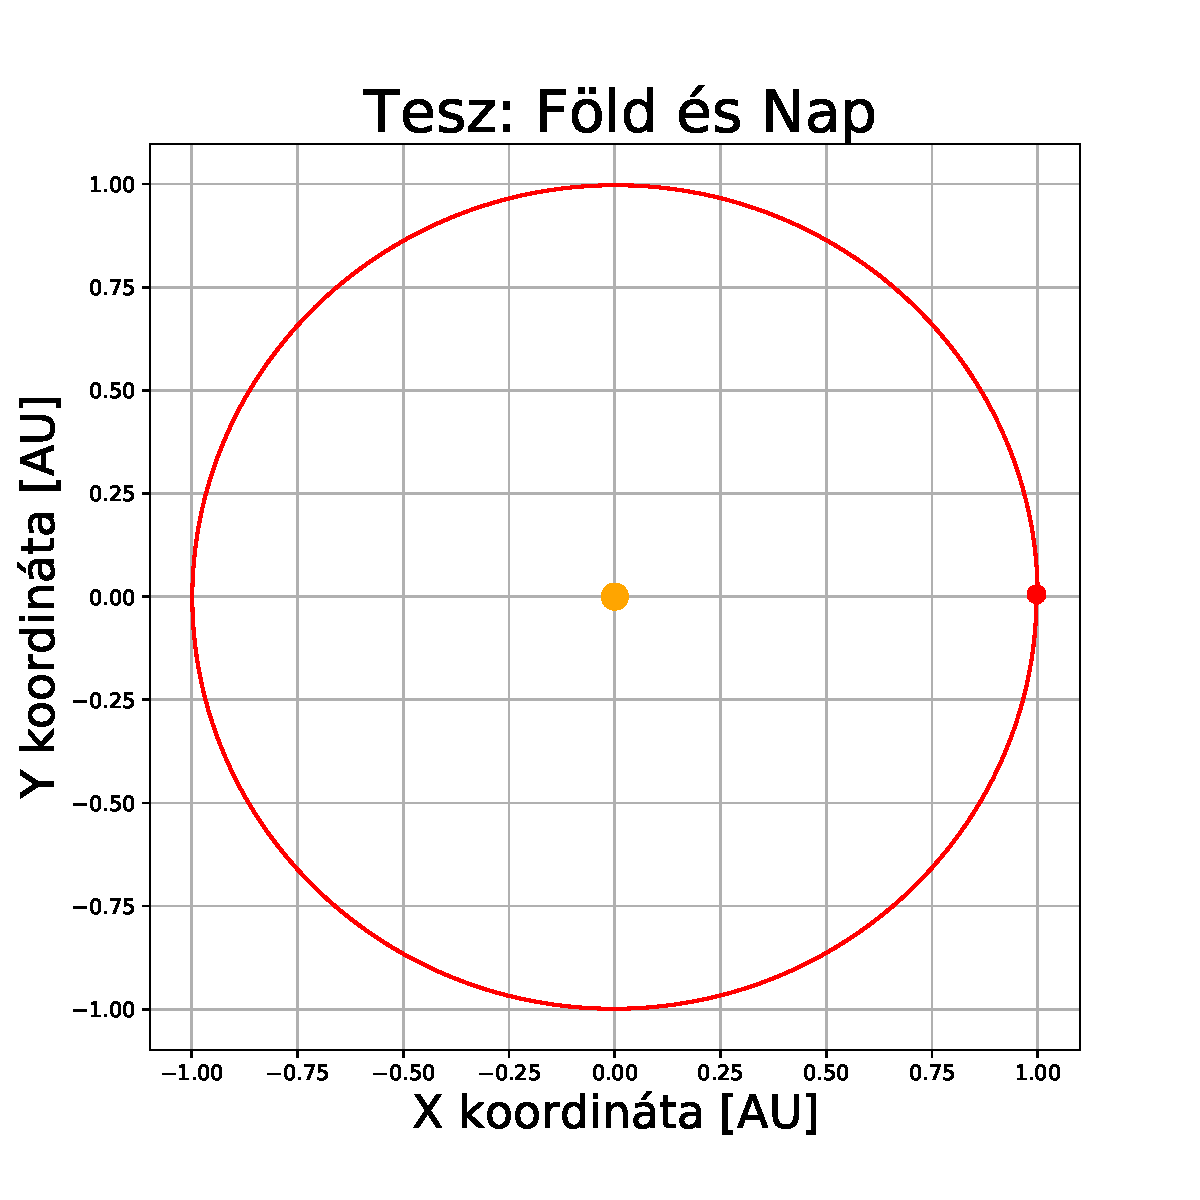
\includegraphics[width=0.7\textwidth]{pics/test1.pdf}
\end{center}
\captionof{figure}{Szimuláció a Földdel és Nappal.}
Láthatóan megfelelő pályát razol ki a fázisdiagram. A szimuláció egy év időtartamot ölel át. Ennek további vizsgálata viszont nem lényeges, hiszen a kinetikus és potenciális energia csak némileg változnak ezen időtartamon. Mivel közel ugyanoda érkezett vissza a bolygó, ezért látható (hosszabb időtartamú szimuláció esetén is) hogy a rendszer energiája megmarad.
Ezen egyszerű teszt megfelelő eredményt adott így egyből tovább is léptem a második tesztre: két csillag és egy bolygó. A "test.txt" tartalmazza ennek az adatait.
\begin{center}
    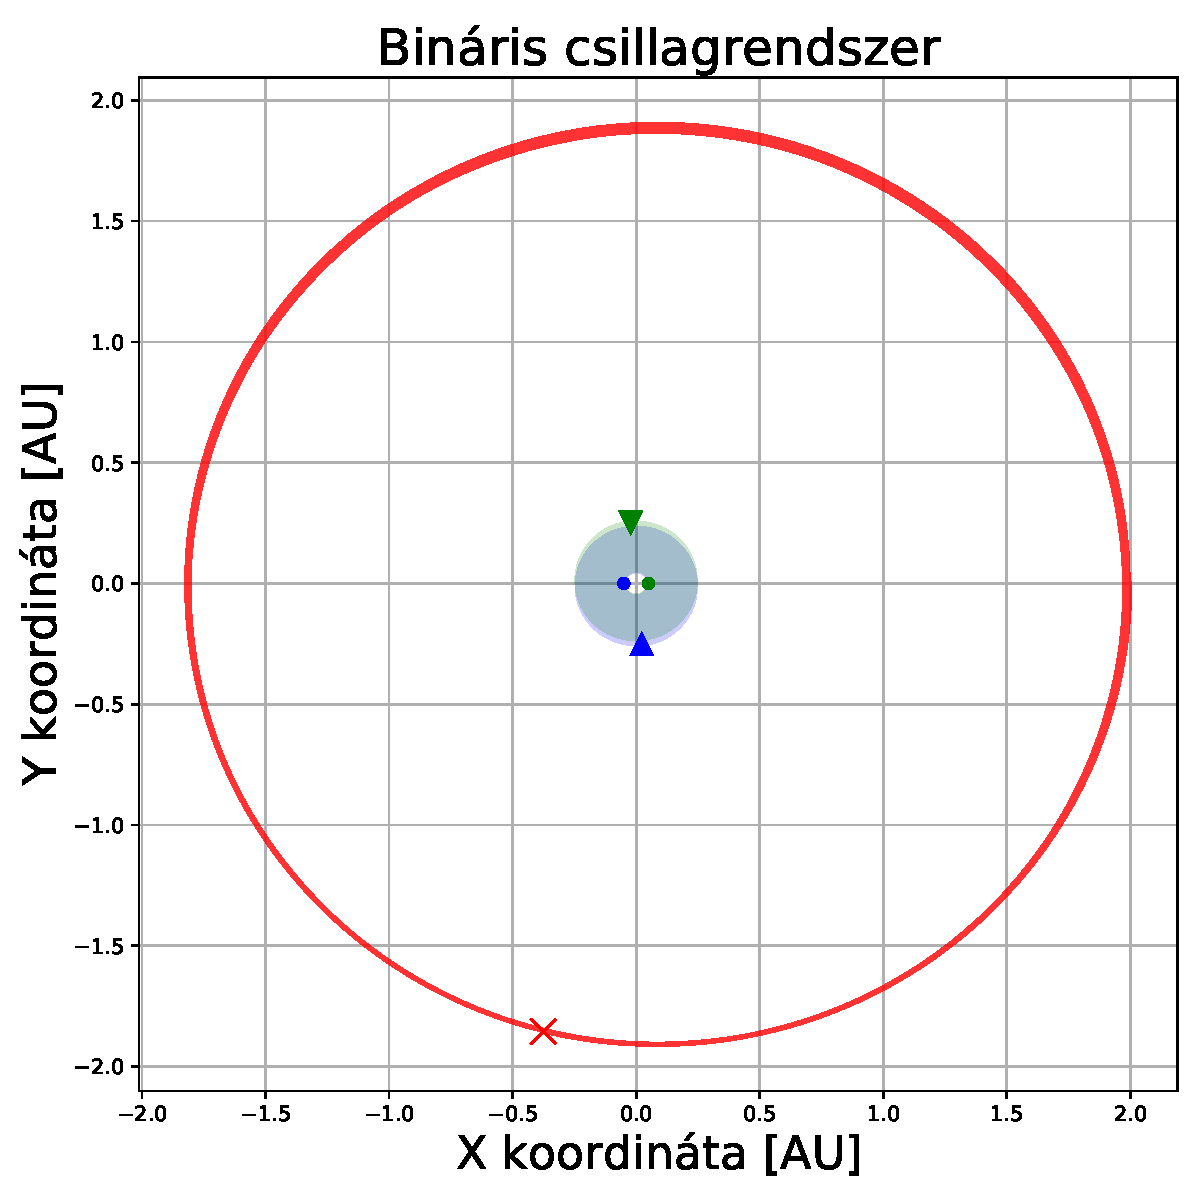
\includegraphics[width=0.7\textwidth]{pics/test2_10.pdf}
    %miért nincs alpha? miért ignorálja ezt az opciót miközben van alpha? még az eredeti képen is jó...!
    \label{fig::binary}
\end{center}
\captionof{figure}{Szimuláció két csillaggal és egy bolygóval. A háromszögek és az x az utolsó állapotot jelöli.}
Az (\ref{fig::binary}) egy sikeres szimulációt jelöl. Látható, hogy a csillagok pályája egy gyűrűt rajzol ki, ami az általuk bejárt területet jelöli. A szimulációhoz szükséges paraméterek megkeresése, ami hosszabb ideig is fennálló stabil rendszert eredményez. Ezek után megtekinthető a rendszer elemeinek eneriája is. 
\begin{center}
    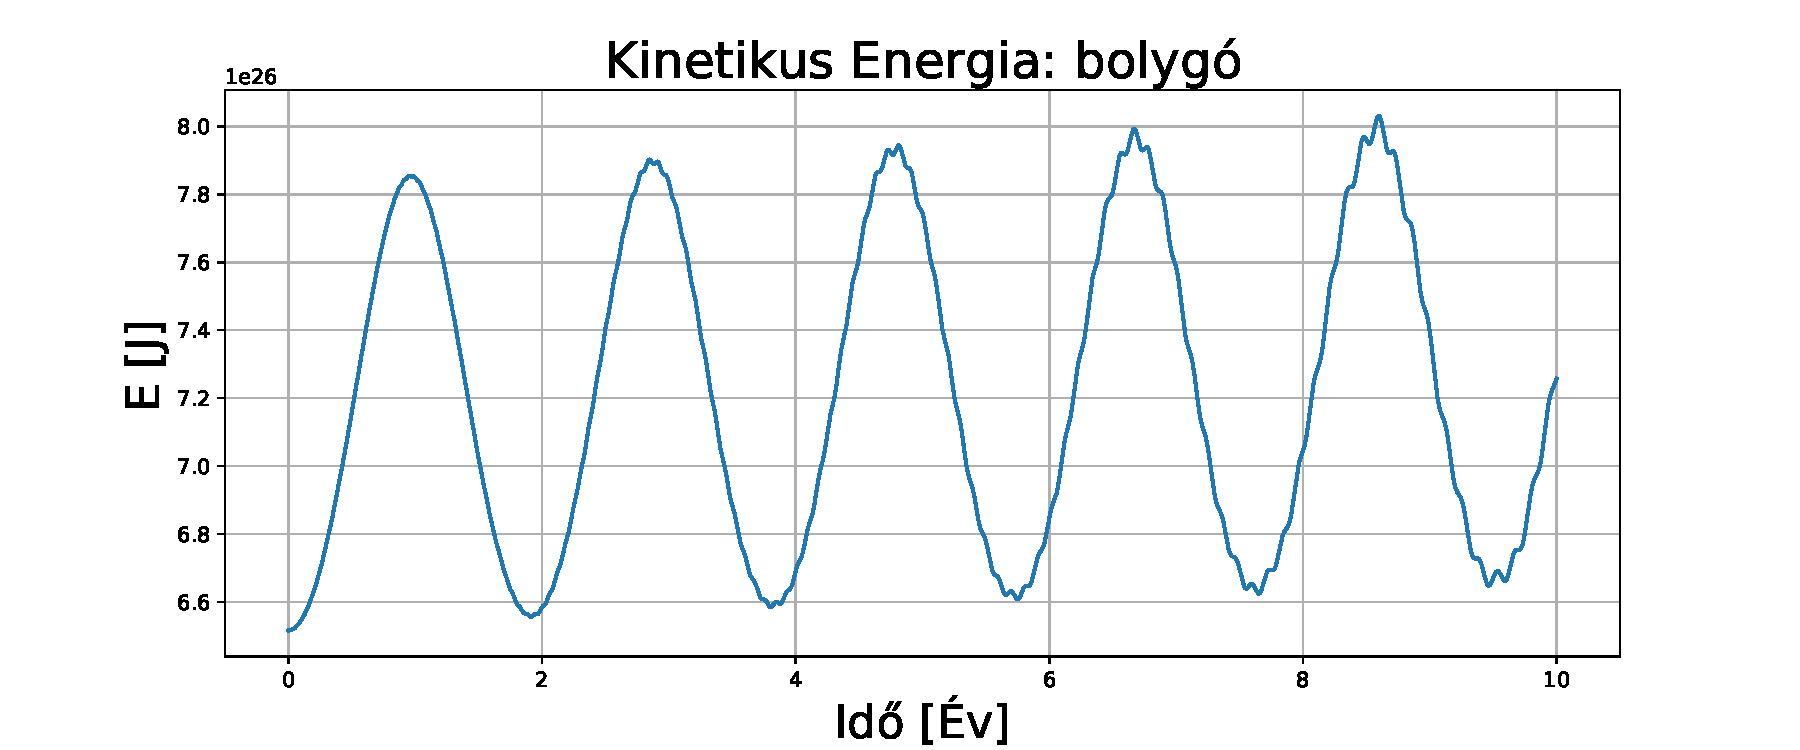
\includegraphics[width=1.1\textwidth]{pics/test2_10BK.pdf}
\end{center}
\begin{center}
    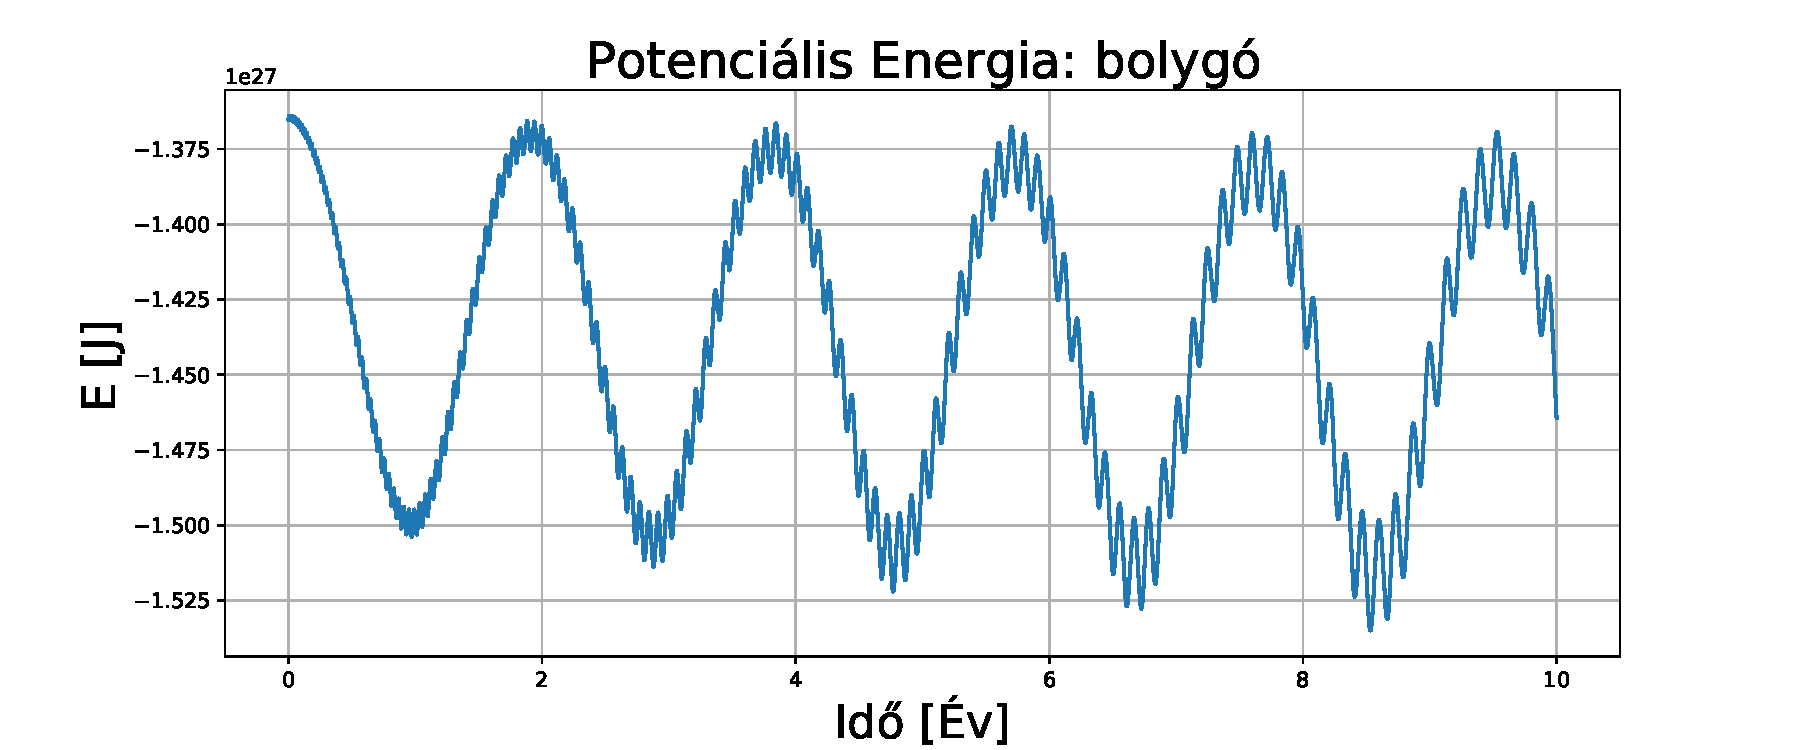
\includegraphics[width=1.1\textwidth]{pics/test2_10BU.pdf}
\end{center}
\begin{center}
    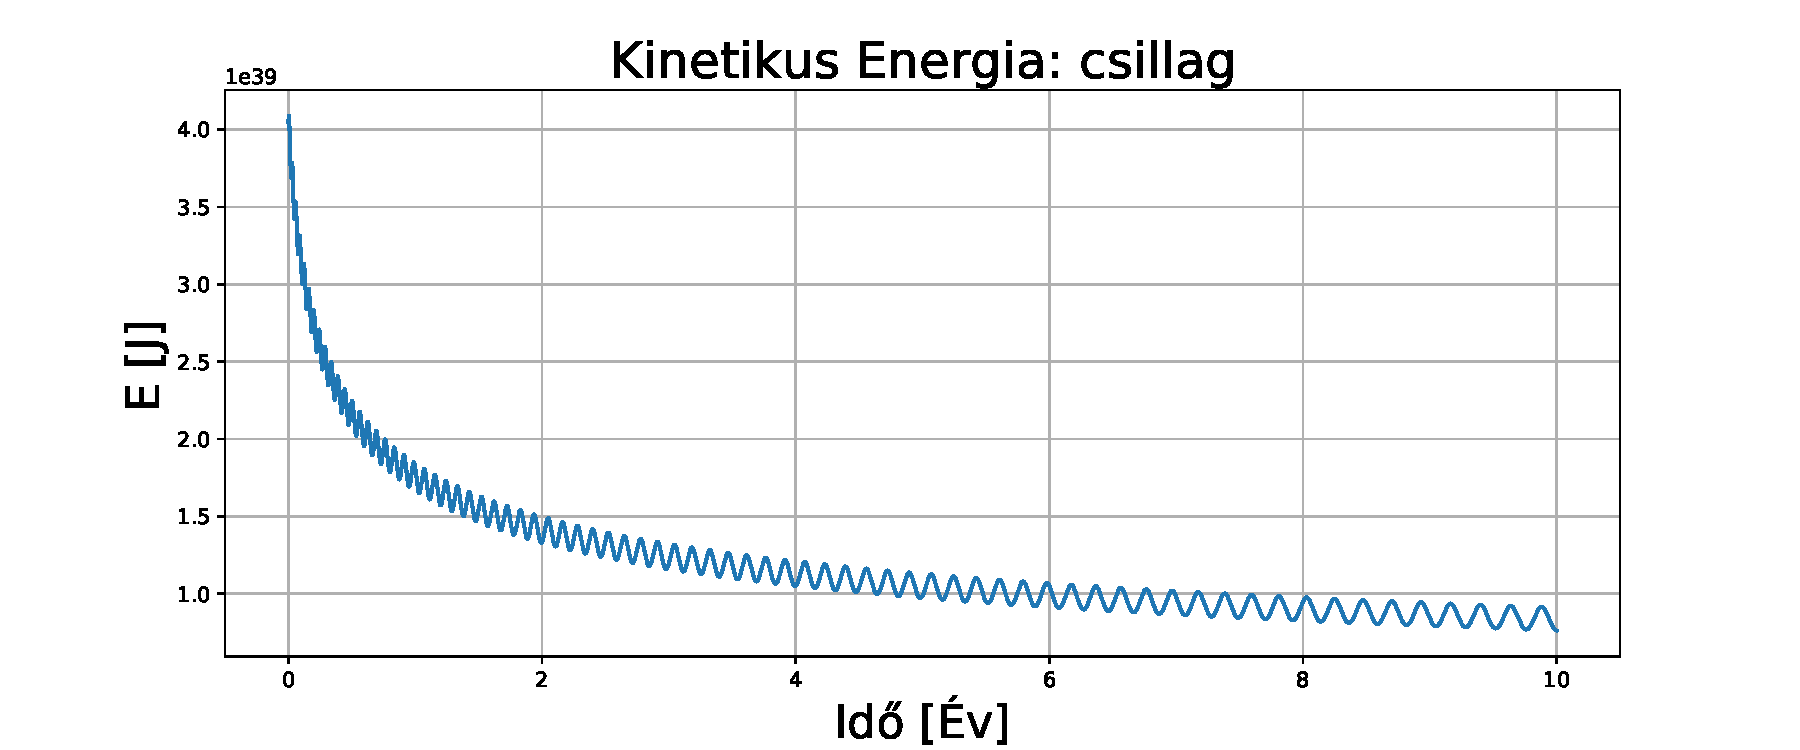
\includegraphics[width=1.1\textwidth]{pics/test2_10CSK.pdf}
\end{center}
\begin{center}
    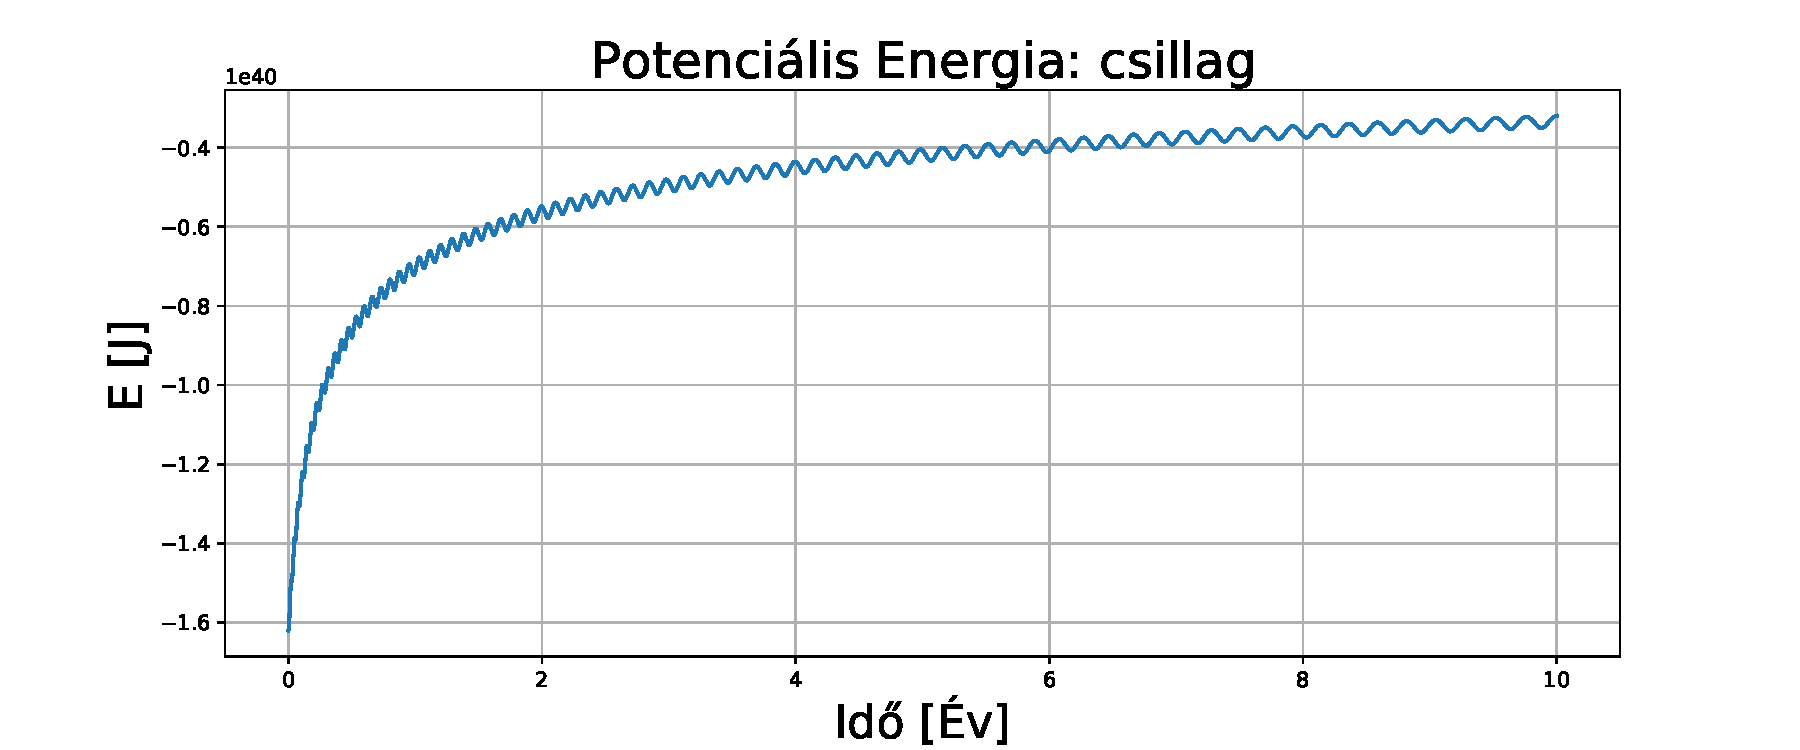
\includegraphics[width=1.1\textwidth]{pics/test2_10CSU.pdf}
\end{center}

Az eredmények egyértelműen rámutatnak a következőekre: A szimuláció során a két csillag mindig eltávolodik egymástól, amire rámutat a kinetikus energia lecsökkenése. A bolygó potenciális energiájának görbéje két jelenségre mutat. Egy teljes periódus alatt is változik az energiája a bolygónak, ahogyan változik a távolsága a rendszer tömegközéppontjától. A máik megfigyelhető jelenség egy szinuszos ingadozás sokkal rövidebb periódus idővel, melynél a periódus hossza és amplitúdója a két csillag közötti távolsággal változik. 

A szimuláció ebben az esetben viszont egy N test szimuláció, így minden test minden másikkal interrakcióbalép.